
% Быть посвободнее при склеивании слов
\sloppy

% Настройка листингов
\renewcommand{\lstlistingname}{Листинг}
\lstset{
	frame=single, % adds a frame around the code
	rulesepcolor=\color{gray},
	rulecolor=\color{black},
	breaklines=true,
	xleftmargin=2em,
	extendedchars={true},
	inputencoding={utf8},
	basicstyle={\ttfamily \scriptsize},
	keywordstyle={\rmfamily \bfseries},
	commentstyle={\rmfamily \itshape},
	tabsize={2},
	numbers={left},
	frame={single},
	showstringspaces={false},
}
\lstdefinestyle{java}{
	breaklines={true},
	texcl=true,
	language={Java},
}
\lstset{
    literate={а}{{\selectfont\char224}}1
    {б}{{\selectfont\char225}}1
    {в}{{\selectfont\char226}}1
    {г}{{\selectfont\char227}}1
    {д}{{\selectfont\char228}}1
    {е}{{\selectfont\char229}}1
    {ё}{{\"e}}1
    {ж}{{\selectfont\char230}}1
    {з}{{\selectfont\char231}}1
    {и}{{\selectfont\char232}}1
    {й}{{\selectfont\char233}}1
    {к}{{\selectfont\char234}}1
    {л}{{\selectfont\char235}}1
    {м}{{\selectfont\char236}}1
    {н}{{\selectfont\char237}}1
    {о}{{\selectfont\char238}}1
    {п}{{\selectfont\char239}}1
    {р}{{\selectfont\char240}}1
    {с}{{\selectfont\char241}}1
    {т}{{\selectfont\char242}}1
    {у}{{\selectfont\char243}}1
    {ф}{{\selectfont\char244}}1
    {х}{{\selectfont\char245}}1
    {ц}{{\selectfont\char246}}1
    {ч}{{\selectfont\char247}}1
    {ш}{{\selectfont\char248}}1
    {щ}{{\selectfont\char249}}1
    {ъ}{{\selectfont\char250}}1
    {ы}{{\selectfont\char251}}1
    {ь}{{\selectfont\char252}}1
    {э}{{\selectfont\char253}}1
    {ю}{{\selectfont\char254}}1
    {я}{{\selectfont\char255}}1
    {А}{{\selectfont\char192}}1
    {Б}{{\selectfont\char193}}1
    {В}{{\selectfont\char194}}1
    {Г}{{\selectfont\char195}}1
    {Д}{{\selectfont\char196}}1
    {Е}{{\selectfont\char197}}1
    {Ё}{{\"E}}1
    {Ж}{{\selectfont\char198}}1
    {З}{{\selectfont\char199}}1
    {И}{{\selectfont\char200}}1
    {Й}{{\selectfont\char201}}1
    {К}{{\selectfont\char202}}1
    {Л}{{\selectfont\char203}}1
    {М}{{\selectfont\char204}}1
    {Н}{{\selectfont\char205}}1
    {О}{{\selectfont\char206}}1
    {П}{{\selectfont\char207}}1
    {Р}{{\selectfont\char208}}1
    {С}{{\selectfont\char209}}1
    {Т}{{\selectfont\char210}}1
    {У}{{\selectfont\char211}}1
    {Ф}{{\selectfont\char212}}1
    {Х}{{\selectfont\char213}}1
    {Ц}{{\selectfont\char214}}1
    {Ч}{{\selectfont\char215}}1
    {Ш}{{\selectfont\char216}}1
    {Щ}{{\selectfont\char217}}1
    {Ъ}{{\selectfont\char218}}1
    {Ы}{{\selectfont\char219}}1
    {Ь}{{\selectfont\char220}}1
    {Э}{{\selectfont\char221}}1
    {Ю}{{\selectfont\char222}}1
    {Я}{{\selectfont\char223}}1
}


% Настройка стиля оглавления
% \renewcommand{\tocchapterfont}{}

%%%%%%%%%%%%%%%%%%%%%%%%%%%%%%%%%%%%%%%%%%%%%%%%%%%%%%%%%%%%%%%%%%%%%%%%%%%%%%%%


\begin{document}


% Заведующий кафедрой
\apname{В.М.~Ицыксон}

% Название
\title{ВЫПУСКНАЯ РАБОТА БАКАЛАВРА}

% Тема
\topic{Разработка учебно-методических средств для исследования моделей глубокого обучения}

% Направление
\coursenum{09.03.01}
\course{Информатика и вычислительная техника}
\masterprognum{09.03.01\_15}
\masterprog{Технологии проектирования системного и прикладного программного обеспечения}

% Автор
\author{Волкова М.Д.}
\group{43501/3}

% Научный руководитель
\sa{Никитин К.В.}
\sastatus{к.~т.~н.,~доц.}

% Рецензент
% \rev{Р.Е.~Цензент}
% \revstatus{к.~т.~н.,~доц.}

% Консультант
%\conspec{нормоконтролю}
%\con{А.Г.~Новопашенный}
%\constatus{к.т.н., доцент}

% Уменьшить размер шрифта для названия института, так как он не влезает в
% одну строчку по новому размеру страницы
\renewcommand\instfont{\small}
% Переопределение названий Университета/Факультета/Кафедры
%\institution{Усть-Гатчинский государственный университет кирпично-велосипедной промышленности}
%\faculty{Институт кройки и шитья}
%\department{Кафедра построения конструкций из пластилина}

\logo{fig/spbpu.jpg}


\def\contentsname{Содержание}

% Contents
\tableofcontents
\clearpage

\section{Цель работы}

Научиться определять оптимальные критерии качества для замкнутой системы.

\section{Программа работы}

\begin{itemize}
	\item Определить область устойчивости
	\item Определить величину статической ошибки.
	\item Получить корневые критерии качества.
	\item Получить частотные критерии качества.
	\item Получить интегральные критерии качества.
	\item Промоделировать процессы в системе при оптимальных параметрах при наличии шума и без.
\end{itemize}

\section{Индивидуальное задание}
Вид управляющего устройства: ПД (изодромное звено).\\
$x'' + 2x' + 0.75x = 0.75u\\
W(p) = \frac{0.75}{p^2 + 2p + 0.75}$

\section{Ход работы}

\subsection{Исходные данные замкнутой системы}

Структура исследуемой системы с добавлением изодромного звена и шума:

\begin{figure}[h!]
	\centering
	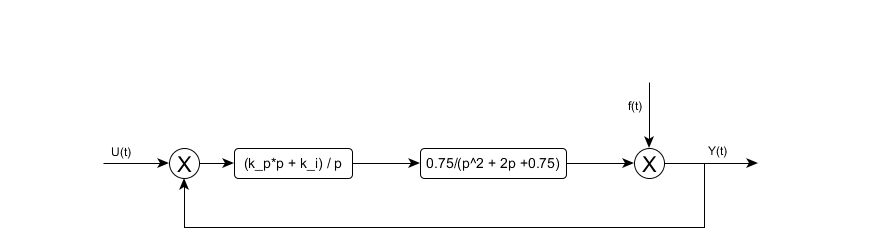
\includegraphics[scale = 0.55]{images/w.png}
	\caption{Структурная схема системы}
	\label{image:1}
\end{figure}

\FloatBarrier
Определим передаточную функцию разомкнутой системы:

$W_p=\frac{k_pp+k_i}{p}\frac{0.75}{p^2 + 2p + 0.75}  =\frac{0.75(k_pp+k_i)}{p(p^2 + 2p + 0.75)}$

Определим характеристический полином замкнутой системы:

$D(p)=B(p)+C(p)=p(p^2 + 2p + 0.75)+0.75(k_pp+k_i)=0.75k_i + 0.75(1 + k_p)p + 2p^2 + p^3$

Определим передаточную функцию замкнутой системы:

$W_3=\frac{W_p}{1 + W_p}=\frac{B(p)}{B(p)+C(p)}=\frac{B(p)}{D(p)}=\frac{0.75(k_pp+k_i)}{Tp^3+(2T+1)p^2+(0.75T+0.75k+2)p+0.75} 
$
%$= \frac{3kp}{4Tp^3+4(2T+1)p^2+(3T+3k+8)p+3}$

\subsection{Определение области устойчивости}

Для выполнения необходимого условия устойчивости системы необходимо, чтобы коэффициенты характеристического полинома были положительны. Для этого должны выполняться следующие условия:

\noindent$
\begin{cases}
	\text{$0.75k_i>0$} \\
	\text{$0.75(1 + k_p)>0$}
\end{cases}
\Longrightarrow
\begin{cases}
	\text{$k_i>0$} \\
	\text{$k_p>-1$}
\end{cases}
$
Для определения достаточного условия устойчивости воспользуемся критерием Гурвица для системы третьего порядка:\\
$a_2a_1-a_3a_0>0$ \\
$2*0.75(1 + k_p)-0.75k_i>0$ \\
$1.5 - 0.75 k_i + 1.5 k_p > 0$ \\


Из неравенства очевидно, что для всех $k_i$ и $k_p$, удовлетворяющих достаточному условию, необходимое условие также соблюдается.

\subsection{Статическая ошибка}

Для данной системы статическая ошибка вычисляется следующим образом:


$e=lim_{t\rightarrow\infty}\frac{U(t)}{1+W_p(t)}$

\noindentТак как система является астатической первого порядка, то $e \rightarrow 0$

\subsection{Корневые критерии качества}

Данная группа критериев применяется для оценки качества системы по корням характеристического полинома:



$D(p)=0.75k_i + 0.75(1 + k_p)p + 2p^2 + p^3$


\textbf{Оценка быстродействия} может производиться на основе величины:


$\Omega=\sqrt[n]{|p_1\cdot...\cdot p_n|}$


Для данной системы существует три корня:

$\Omega=\sqrt[3]{|p_1\cdot p_2\cdot p_3|}=\sqrt[3]{-0.75k_i}$
Видно, что система достигнет наилучшего быстродействия при значении $k_i = 0$.

\textbf{Степень устойчивости} системы определяется как абсолютное значение действительной части корней, ближайших к мнимой оси корня (к нулю):

$realPart = min(|Re(p_1)|, |Re(p_2)|, |Re(p_3)|)$

Таким образом, для получения оптимальных параметров $k_i$ и $k_P$, значение $realPart$ нужно минимизировать. В результате минимизации получились значения $k_i = 0$ и $k_p = 100$. 
Значения корней при полученных значениях параметров:

$\begin{cases}
 p_1 = 0\\p_2 = -1 + 8j\\ p_3 = -1 -8j 
 \end{cases}
 $

\textbf{Колебательность системы} определяется мнимыми частями корней. Для нулевой колебательности все мнимые части корней должны быть равны нулю.
Таким образом, для получения оптимальных параметров $k_i$ и $k_p$, должно быть выполнено условие:

$\begin{cases}
Imagine(p_1)=0\\Imagine(p_2)=0\\Imagine(p_3)=0
\end{cases}
$

Так как условие не выполняется, можно сказать, что при полученных значениях параметров
в системе имеется колебательность.

\subsection{Частотные критерии качества}

Для оценки качества системы по частотным критериям представим передаточную функцию в частотном виде:

\noindent$W_3(j\omega)= Re(\omega)+ j Im(\omega)$\\
$Denom(\omega) = (- 8\omega^2 + 3k_i)^2 + (- 4\omega^3 + (3k_p + 3)\omega)^2$\\
$Re(\omega) = \frac{3k_i(- 8\omega^2 + 3k_i)}{Denom(\omega)} + \frac{3k_p\omega(- 4\omega^3 + (3k_p + 3)\omega)}{Denom(\omega)}$\\
$Im(\omega) = \frac{3k_p\omega(- 8\omega^2 + 3k_i)}{Denom(\omega)} - \frac{3k_i(- 4\omega^3 + (3k_p + 3)\omega)}{Denom(\omega)}$\\
$A(\omega) = \sqrt{Re(\omega)^2 + Im(\omega)^2} = 
\frac{3\sqrt{k_i^2 + k_p^2\omega^2}}{\sqrt{9k_i^2 - 48k_i\omega^2 + 9k_p^2\omega^2 - 24k_p\omega^4 + 18k_p\omega^2 + 16\omega^6 + 40\omega^4 + 9\omega^2}}$

\textbf{Показатель колебательности} определяется как отношение максимального модуля АЧХ к его значению при нулевой частоте:

$M=\frac{max(A(\omega))}{A(0)} = max(A(\omega))$
Показатель колебательности характеризует склонность систем или объектов к колебательности. Чем выше показатель колебательности, тем более колебательна система, то есть менее
качественна.
Так как значение АЧХ при нулевой частоте равно единице для любых значений $k_i$ и $k_p$, то 
для получения оптимальных параметров необходимо найти минимум функции $max(A(\omega))$. 
Для рассчитанных оптимальных параметров $k_i = 0$ и $k_P = 100$ значение колебательности $M = 4.33$ (достигается на частоте $\omega = 8.60$).

\textbf{Запас устойчивости по амплитуде} определяется следующим образом:

$C=\frac{M^2}{M^2-1}$

При оптимальных значениях параметров запас устойчивости по амплитуде составляет $C = 1.05$

\textbf{Запас устойчивости по фазе} определяется следующим образом:

$\mu=arccos(1-\frac{M^2}{2})$

\noindentПри оптимальных значениях параметров запас устойчивости по фазе составляет\\ $\mu = \pi - 2.81j$

\textbf{Полоса пропускания}

$0 < \omega < 13.35$


\subsection{Интегральные критерии качества}

Воспользуемся квадратичным критерием качества:

$I=\int_{0}^{\infty}x^2(t)dt$

Для данной системы $x^2(t)=(h(t)-1(t))^2$, где $h(t)$ - переходная характеристика замкнутой системы, а $1(t)$ - входное воздействие:


$I=\int_{0}^{\infty}(h(t)-1(t))^2dt$

Таким образом, для получения оптимальных параметров $k_i$ и $k_p$, значение $I$  нужно минимизировать. Полученные значения параметров $k_i = 0$ и $k_p = 100$. Значение интеграла при этом $I = 0.25$. 

\subsection{Анализ полученной системы}

В качестве оптимальных параметров были выбраны параметры, полученные на основе
интегрального критерия качества  $k_i = 0$ и $k_p = 100$.

\begin{figure}[h!]
	\centering
	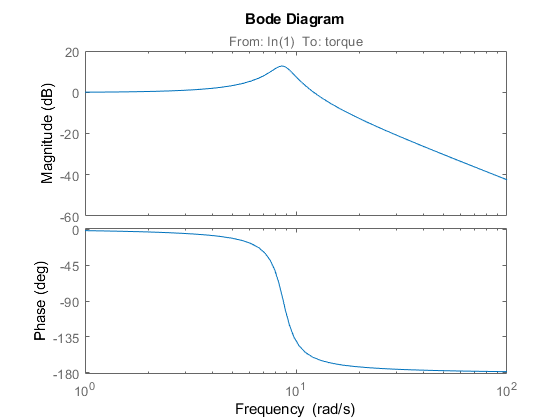
\includegraphics[scale = 0.70]{images/bode.png}
	\caption{Диаграмма боде полученной системы}
	\label{image:9}
\end{figure}

\FloatBarrier

Выясним, как будет вести себя система при наличии шума. В этом случае
дифференциальное уравнение приобретает следующий вид:
$D(p)x(t) = B(p)g(t) + N(p)f(t)$, где $f(t)$ - сигнал шума, $N(p)/D(p)$ - передаточная
функция системы по шуму.
Выберем в качестве шума единичную функцию Гаусса (Белый шум) $N(p) = 1$.
При моделировании получим следующий результат:

\begin{figure}[h!]
	\centering
	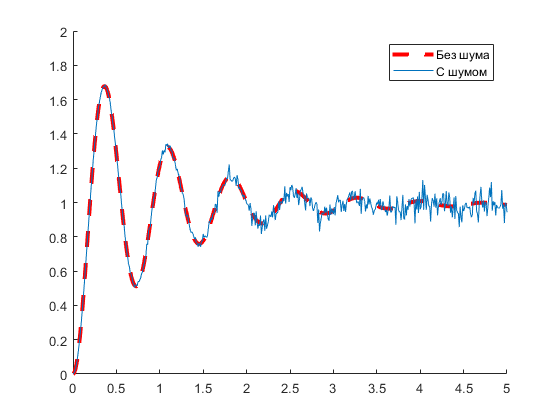
\includegraphics[scale = 0.70]{images/result.png}
	\caption{Реакция системы на функцию Хэвисайда}
	\label{image:9}
\end{figure}
\FloatBarrier
Видно, что в промежуток времени, когда значение выходного сигнала возрастает, наличие шума практически не сказывается на поведении системы. Наибольшее
влияние обнаруживается, когда после этого система устремляется к значению в установившемся режиме. Также на графике видна колебательность системы.

\section{Вывод}

При использовании изодромного звена в качестве управляющего устройства, оптимальные параметры не удалось установить однозначным образом.  Параметры были выбраны согласно
интегральному критерию качества.

По значениям корней можно сделать вывод, что система находится на апериодической границе
устойчивости. Также можно сказать, что в системе присутствует колебательность. Это
подтверждается результатами на графике.

Стоит отметить, что описанные правила для выбора $k_i$ и $k_p$ справедливы для только ОУ с конкретной переходной характеристикой, в то время как для других ОУ эти значения должны рассчитываться отдельно.

\end{document}
